\section{Zustandsraumdarstellung \formelbuch{139} \tiny{$Revision: 1352 $}}
\scriptsize
Darstellung einer Differentialgleichung $n$. Ordnung durch ein
Differentialgleichungssystem von $n$ Gleichungen 1. Ordnung.

\subsection{Definition \formelbuch{140}}
\begin{tabular}{ll}
\parbox{10cm}{
	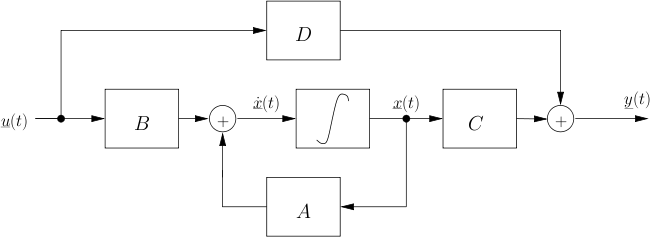
\includegraphics[width=10cm]{./bilder/zrd-schema.png}
	}
	& \parbox{8cm}{
		$\dot{\underline{x}}(t) = {\boldsymbol A} \underline{x}(t) + {\boldsymbol B}
		\underline{u}(t)$ \\
		$\underline{y}(t) = {\boldsymbol C} \underline{x}(t) + {\boldsymbol D}
		\underline{u}(t)$\\ 
		
		${\boldsymbol A}$: Systemmatrix ($n$ x $n$): Spalten entsprechen Ausgängen
		der Integratoren, Zeilen Eingänge ; \\ 
		${\boldsymbol B}$: Steuer- oder
		Eingangsmatrix ($n$ x $m$) ``senkrecht''; \\ ${\boldsymbol C}$: Beobachtungs- oder Ausgangsmatrix ($k$ x $n$)
		``waagrecht''; \\
		${\boldsymbol D}$: Übergangs- oder Durchgangsmatrix ($k$ x
		$m$)\\
		
		wobei $m$ der Anzahl Eingangssignale, $k$ der Anzahl Ausgangssignale \& $n$ der
		Anzahl Zustandsgrössen (Integratoren, Ordnung) entsprechen.\\
	}
 \end{tabular}


\subsection{ZRD im Frequenzbereich \formelbuch{147} \matlab{ss2tf}}
$$\boldsymbol{H(s)} = \frac{\underline{Y}(s)}{\underline{U}(s)} =
\boldsymbol{C}\left(s\boldsymbol{I_n}-\boldsymbol{A}\right)^{-1}\boldsymbol{B}+\boldsymbol{D}$$
\\
Die Grösse der Matrix $\boldsymbol {H(s)}$ entspricht der Grösse der
Durchgangsmatrix $\boldsymbol D$. $\boldsymbol{I_n}$ sei die Einheitsmatrix mit
Grösse $n$ x $n$.

\subsection{Übertragungsmatrizen \formelbuch{149}}
$$H(s)=\frac{Y(s)}{U(s)}=\frac{b_{m} s^{m} + b_{m-1} s^{m-1} +\cdots+b_{1} s 
+ b_{0}}{s^{n} + a_{n-1} s^{n-1} + \cdots + a_{1} s + a_{0}}$$\\
Allgemeine Formel für $m=1$ Eingang, $k=1$ Ausgang, $n=2$ Integratoren:\\
$$H(s) = \left [ 
\begin{array}{c c}
C_{11}  & C_{12}\\
\end{array}
\right ]\cdot
\left (
\left [ 
\begin{array}{cc}
 s & 0\\
0 & s\\
\end{array}
\right ] -
\left [ 
\begin{array}{cc}
 A_{11} & A_{12}\\
 A_{21} & A_{22}\\
\end{array}
\right ]
\right )^{-1}\cdot
\left [ 
\begin{array}{c}
 B_{11}\\
 B_{21}\\
\end{array}
\right ]+ D$$
$$=  \frac{B_{11}C_{11}(s-A_{22}) + B_{11}C_{12}A_{21} +
B_{21}C_{11}A_{12} + B_{21}C_{12}(s-A_{11})}{(s-A_{22})(s-A_{11}) - A_{12}A_{21}} + D$$


\subsection{Stabilität \formelbuch{153}}
Wenn alle Realteile der Eigenwerte $\lambda$ der Systemmatrix ${\boldsymbol A}$
negativ sind, ist ein LTI-System asymptotisch stabil, jedoch nicht umgekehrt:
$\left | \lambda\boldsymbol{I} - \boldsymbol{A} \right |   =0 \rightarrow \forall~\lambda \quad\Re \{\lambda\}<0$

\subsection{Beobachtbar- \& Steuerbarkeit \formelbuch{154}}
\subsubsection{Steuerbarkeit \matlab{ctrb}}
Gibt es Zustände von $\underline{x} (t)$ die nicht von den
Eingängen $\underline{u} (t)$ beeinflusst werden? Wenn ja,
dann ist das System nicht steuerbar!

Wenn $|Q_{Steuerbarkeit}|= \left| \left [ \boldsymbol{B~~AB~~ A^2B~\ldots~
A^{n-1}B} \right ] \right|  \neq 0$, dann ist das System vollständig steuerbar.


\subsubsection{Beobachtbarkeit \matlab{obsv}}
Gibt es Zustände $\underline{x}(t)$ die keinen Einfluss auf die Ausgänge
$\underline{y}(t)$ haben? Wenn ja, kann man aus dem Verhalten von 
$\underline{y}(t)$ nicht auf die Zustände $\underline{x}(t)$ schliessen!
Das System ist nicht beobachtbar!


Wenn $|Q_{Beobachtbarkeit}| = \left| \left [ \boldsymbol{
\begin{array}{c}
 C\\
 CA\\
CA^2\\
\vdots \\
CA^{n-1}\\
\end{array}}\right ] \right| \neq 0$, dann ist das System vollständig
beobachtbar.

\subsubsection{Regelungsnormalform \formelbuch{150}}
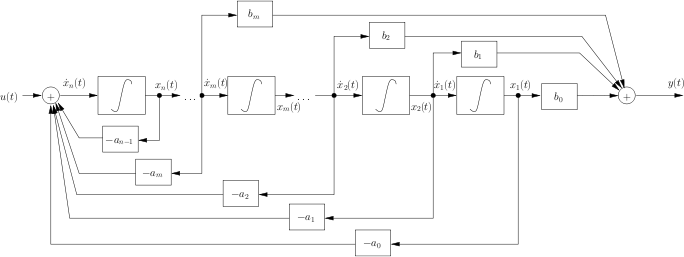
\includegraphics[width=10cm]{./bilder/zrd-regelungsnormalform.png} \\
\scriptsize
\begin{equation*}
\left [ 
\begin{array}{c}
\dot{x}_1(t)\\
\dot{x}_2(t)\\
\vdots\\
\dot{x}_{n-1}(t)\\
\dot{x}_{n}(t)\\
\end{array}
\right ] =
\left [ 
\begin{array}{c c c c c}
0 & 1 & 0 & \ldots & 0\\
0 & 0 & 1 & \ldots & 0\\
\vdots & \vdots & \vdots & \ddots & \vdots\\
0 & 0 & 0 & \ldots & 1\\
-a_0 & -a_1 & -a_2 & \ldots & -a_{n-1}\\
\end{array}
\right ]\cdot
\left [ 
\begin{array}{c}
x_1(t)\\
x_2(t)\\
\vdots \\
x_{n-1}(t)\\
x_{n}(t)\\
\end{array}
\right ]+
\left [ 
\begin{array}{c}
0 \\
0\\
\vdots\\
0\\
1\\
\end{array}
\right ]\cdot
u(t),
\end{equation*}
\begin{equation*}
y(t) = 
\left [ 
\begin{array}{c c c c}
b_0-a_0b_n & b_1-a_1b_n & \ldots & b_{n-1}-a_{n-1}b_n\\
\end{array}
\right ] \cdot
\left [ 
\begin{array}{c}
x_1(t)\\
x_2(t)\\
\vdots \\
x_{n-1}(t)\\
x_{n}(t)\\
\end{array}
\right ]+
\left [ 
\begin{array}{c}
b_n \\
\end{array}
\right ] \cdot
u(t).
\end{equation*}
\normalsize


\subsubsection{Beobachtungsnormalform \formelbuch{151}}
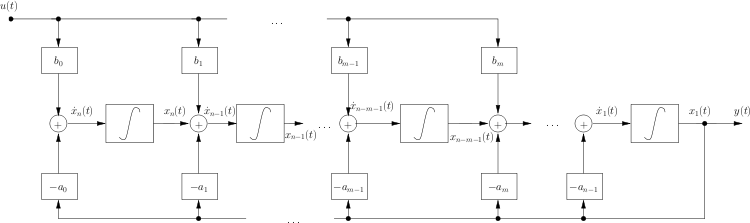
\includegraphics[width=10cm]{./bilder/zrd-beobachtungsnormalform.png} \\
\scriptsize
\begin{eqnarray*}
\left [ 
\begin{array}{c}
\dot{x}_1(t)\\
\dot{x}_2(t)\\
\vdots\\
\dot{x}_{n-1}(t)\\
\dot{x}_n(t)\\
\end{array}
\right ] &=&
\left [ 
\begin{array}{c c c c c}
0 & 0 & 0 & \ldots & -a_0\\
1 & 0 & 0 & \ldots & -a_1\\
0 & 1 & 0 & \ldots & -a_2\\
\vdots & \vdots &  \ddots & 0 & \vdots\\
0 & 0 & \ldots & 1 & -a_{n-1}\\

\end{array}
\right ]\cdot
\left [ 
\begin{array}{c}
x_1(t)\\
x_2(t)\\
\vdots \\
x_{n-1}(t)\\
x_{n}(t)\\
\end{array}
\right ]+
\left [ 
\begin{array}{c}
b_0-a_0b_n \\
b_1-a_1b_n\\
b_2-a_2b_n\\
\vdots\\
b_{n-1}-a_{n-1}b_n\\
\end{array}
\right ]\cdot
u(t),\\
y(t) &= &
\left [ 
\begin{array}{c c c c}
0 & 0 & \ldots & 1\\
\end{array}
\right ] \cdot
\left [ 
\begin{array}{c}
x_1(t)\\
x_2(t)\\
\vdots \\
x_{n-1}(t)\\
x_{n}(t)\\
\end{array}
\right ]+
\left [ 
\begin{array}{c}
b_n \\
\end{array}
\right ] \cdot
u(t).
\end{eqnarray*}
\normalsize
